\documentclass[10pt]{amsart}
\usepackage[a4paper,margin=23mm]{geometry}
\usepackage{amsmath,amssymb,amsthm,mathtools,enumitem,hyperref,graphicx,xspace}
\usepackage[english]{babel}
\newcommand{\resp}{resp.}\newcommand{\cf}{cf.}\newcommand{\ie}{i.e.}\newcommand{\eg}{e.g.}
\newcommand{\loccit}{loc.\ cit.}\newcommand{\skpt}{\par\smallskip\noindent}
\emergencystretch=3em\pagestyle{plain}
\newtheorem{theorem}{Theorem}[section]
\newtheorem{prop}[theorem]{Proposition}
\newtheorem{lemma}[theorem]{Lemma}
\newtheorem{coro}[theorem]{Corollary}
\newenvironment{theo}{\begin{theorem}}{\end{theorem}}
\usepackage{letltxmacro}
\LetLtxMacro\sourceenumerate\enumerate
\LetLtxMacro\endsourceenumerate\endenumerate
\renewenvironment{enumerate}[1][]{\if\relax\detokenize{#1}\relax\sourceenumerate\else\sourceenumerate[label=#1]\fi}{\endsourceenumerate}
\usepackage{bbm}
\usepackage[linesnumbered,lined,ruled]{algorithm2e}
%\usepackage{mathrsfs} 
%\usepackage{stmaryrd}

\newcommand\boxempty{\mathrel{\square}}


\DeclarePairedDelimiter\abs{\lvert}{\rvert} 

\newcommand{\mathscr}[1]{\mathcal{#1}}

%%%%%%%%%%%%%%
\DeclareMathOperator{\gon}{gon}
\DeclareMathOperator{\val}{val}
\DeclareMathOperator{\tw}{tw}
\DeclareMathOperator{\Aut}{Aut}
\DeclareMathOperator{\Div}{Div}
\DeclareMathOperator{\supp}{supp}
\DeclareMathOperator{\Prin}{Prin}
\DeclareMathOperator{\Jac}{Jac}
\DeclareMathOperator{\outdeg}{outdeg}
\DeclareMathOperator{\Red}{Red}
\DeclareMathOperator{\ggon}{ggon}
%\text{ggon}


%%%%%%%%%%%%%%%%%%%%%%%%%%%%%%%%%%%%%
\newcommand*{\mk}{\mkern -1mu}
\newcommand*{\Mk}{\mkern -2mu}
\newcommand*{\mK}{\mkern 1mu}
\newcommand*{\MK}{\mkern 2mu}

\hypersetup{urlcolor=purple, linkcolor=blue, citecolor=red}


\newcommand*{\romanenumi}{\renewcommand*{\theenumi}{\roman{enumi}}}
\newcommand*{\Romanenumi}{\renewcommand*{\theenumi}{\Roman{enumi}}}
\newcommand*{\alphenumi}{\renewcommand*{\theenumi}{\alph{enumi}}}
\newcommand*{\Alphenumi}{\renewcommand*{\theenumi}{\Alph{enumi}}}
%%%%%%%%%%%%%%%%%%%%%%%%%%%%%%%%%%




%%%%%%%%%%%%%%%%%%%%%%%%%%%%%%%%%%%%%%%%%%%
%%%%% Auteurs
\begin{document}
\title{Order-three tree-quotient automorphisms from zero-three divisors on simple 3-vertex-connected graphs}
\author{Ivan Aidun \and Frances Dean \and Ralph Morrison \and Teresa Yu \and Julie Yuan}
\maketitle
\section{Graph divisors and harmonic maps}
We define a \emph{graph} $G = (V, E)$ with vertex set $V(G)$ and edge set $E(G)$ to be a finite, connected, loopless, multigraph. Throughout this paper, all graphs are assumed to be combinatorial (that is, without lengths assigned to edges) unless otherwise stated. Graphs with no multiple edges are called \emph{simple}. Given a vertex $v \in V(G)$ and an edge $e \in E(G)$, we use the notation $v \in e$ to indicate that $v$ is an endpoint of $e$. For $u,v \in V(G)$, define $E(u,v) \coloneqq \{ e \in E(G) : u \in e, v \in e\}$. Similarly, for $A, B \subset V(G)$ define $E(A, B) \coloneqq \{ e \in E(G) : e \in E(a, b) \; \text{for some} \; a \in A, b \in B\}$. The \emph{valence} of a vertex $v \in V(G)$ is defined as $\val (v) \coloneqq |\{ e \in E(G) : v \in e \}|$. We define the \emph{genus} of a graph $G$ as $g(G) \coloneqq |E(G)| - |V(G)| + 1$. A graph of genus 0 is called a \emph{tree}.

A graph $G = (V, E)$ is \emph{$k$-edge-connected} if, for any set $W$ of $k-1$ edges, the subgraph $(V,E-W)$ is connected. We let $\eta(G)$ denote the \emph{edge-connectivity} of the graph. That is, $\eta(G)$ is the maximum integer $k$ such that $G$ is $k$-edge-connected. A \emph{bridge} of $G$ is an edge whose deletion strictly increases the number of connected components of $G$. A graph is \emph{bridgeless} if it has no bridges, or equivalently if it is $2$-edge-connected.

Similarly, a graph $G = (V, E)$ is \emph{$k$-vertex-connected} (or just \emph{$k$-connected}) if, for any set $U$ of $k-1$ vertices, the subgraph $(V-U,E)$ is connected. We let $\kappa(G)$ denote the \emph{vertex-connectivity} of the graph. That is, $\kappa(G)$ is the maximum integer $k$ such that $G$ is $k$-vertex-connected. (By convention, we set $\kappa(G)=|V|-1$ if every pair of vertices in $G$ is joined by an edge.) Since removing a vertex from a graph removes all edges incident to that vertex, we have that $\kappa(G)\leq \eta(G)$ for any graph $G$.

\subsection{Divisor Theory on Graphs}

We now review the key concepts of divisor theory on graphs, as developed in~\cite{baker}. A \emph{divisor} $D$ on a graph $G$ is a $\mathbb{Z}$-linear combination of vertices. We will often explicitly write out divisors with the notation
\[
D = \sum_{v \in V(G)} D(v) \cdot (v),
\]
where $D(v)$ denotes the value of $D$ at $v$.
The set of all divisors $\Div (G)$ on a graph $G$ forms an abelian group under component-wise addition. The \emph{degree} of a divisor $D$ is defined as the sum of its integer coefficients:
\[
\deg (D) \coloneqq \sum_{v \in V(G)} D(v).
\]

For a fixed $k \in \mathbb{Z}$, let $\Div ^k(G)$ be the set of all divisors of degree $k$ on $G$. A divisor $D$ is \emph{effective} if, for all $v \in V(G)$, $D(v) \geq 0$. Let $\Div _+(G)$ be the set of all effective divisors on a graph $G$ and for $k \in \mathbb{Z}_{>0}$, let $\Div _+^k(G)$ be the set of all effective divisors of degree $k$ on $G$. For a given effective divisor $D$, we define the \emph{support} of $D$ as
\[
\supp (D) \coloneqq \{ v \in V(G) : D(v) > 0 \}.
\]

The \emph{Laplacian} $\mathcal{L}(G)$ of a graph $G$ is the $|V|\times |V|$ matrix with entries
\[
\mathcal{L}_{v,w} = 
\begin{cases}
\val (v) \quad &\text{if $v = w$} \\
-| E(v, w) | \quad &\text{if $v \neq w$}.
\end{cases}
\]
We use $\Delta : \Div (G) \to \Div (G)$ to denote the \emph{Laplace operator} associated with the Laplacian matrix. A \emph{principal divisor} is a divisor in the image of $\Delta$. We use $\Prin (G)$ to denote the set of principal divisors on a graph $G$, \ie $\Prin (G) = \Delta(\Div (G))$. Notice that $\Prin (G)$ is a normal subgroup of $\Div ^0(G)$. We can therefore define the \emph{Jacobian} $\Jac (G)$ of a graph $G$ as the quotient group $\Div ^0(G) / \Prin (G)$.

Now, define an equivalence relation $\sim$ on divisors such that $D \sim E$ if and only if $D - E \in \Prin (G)$. We say in this case that $D$ and $E$ are \emph{linearly equivalent} and define the \emph{linear system} associated with a divisor $D$ as
\[
|D| \coloneqq \{ E \in \Div _+(G) : E \sim D \}.
\]
For a divisor $D \in \Div (G)$, we define the \emph{rank} of $D$ as $r(D) \coloneqq -1$ if $|D| = \varnothing$, and otherwise as
\[
r(D) \coloneqq \max \{ k \in \mathbb{Z} : |D - F| \neq \varnothing \; \text{for all} \; F \in \Div _+^k(G) \}.
\]
The \emph{gonality} of a graph $G$ is defined as
\[
\gon (G) \coloneqq \min \{ \deg (D) : D \in \Div _+(G), r(D) \geq 1 \}.
\] Later, when we need to distinguish between two different types of gonality, this will be referred to as \emph{divisorial gonality}.

\subsection{Baker--Norine Chip--Firing}

The definition of gonality provided in the previous section has an equivalent statement in terms of chip-firing games on graphs. In a chip-firing game, we think about placing integer numbers of poker chips on the vertices of our graph. A negative number of poker chips corresponds to a vertex being ``in debt''. A \emph{chip-firing move} involves selecting a vertex $v \in V(G)$, subtracting $\val (v)$ chips from $v$, and adding $|E(v,v')|$ chips to each $v'$ adjacent to $v$.

The \emph{Baker--Norine chip-firing game} is played with the following rules:

\begin{enumerate}
 \item\label{sect2.2_1} One player places $k$ chips on the vertices $V(G)$ of a graph $G$ in any arrangement.
 \item\label{sect2.2_2} Another player (the adversary) chooses a vertex $v \in V(G)$ from which to subtract a chip, possibly putting $v$ into debt.
 \item\label{sect2.2_3} The first player wins if they can reach a configuration of chips where no vertex is in debt via a sequence of chip-firing moves. Otherwise, the adversary wins.
\end{enumerate}

Notice that these ``chip configurations'' correspond to divisors on graphs. By standard results as in~\cite{bn}, chip-firing moves correspond to subtracting principal divisors; the divisors present before and after chip-firing are equivalent; and the gonality of a graph is equivalent to the minimum number of chips $k$ required to guarantee that the first player has a winning strategy in the Baker--Norine chip-firing game. Hence, we define a \emph{winning divisor} $D$ to be a divisor satisfying $r(D) \geq 1$. 

Since chip-firing is a commutative operation, we can chip-fire from an entire subset $A \subset V(G)$ at once by sending a chip along each edge outgoing from the subset. Let $\mathbbm{1}_A$ denote the indicator vector on $A$. Then, given a divisor $D$, the resulting divisor after chip-firing from the subset $A$ is $D - \Delta \mathbbm{1}_A$. We define the \emph{outdegree} of $A$ from a vertex $v \in A$ to be the number of edges leaving $A$ from $v$, so
\[
\outdeg _v(A) \coloneqq | E(\{v\}, V(G) - A) |.
\]
Hence, a chip-firing move from a subset $A \subset V(G)$ sends $\outdeg _v(A)$ chips from each vertex $v \in A$ into $V(G) - A$. The total outdegree of $A$ is defined as $\outdeg _A(A) \coloneqq \sum_{v \in A} \outdeg _v(A)$. The following result is proven in~\cite{db}.

\begin{lemma}
\label{lemma:finiteseq}
Given an effective divisor $D$ and an equivalent effective divisor $D'$, there exists a finite sequence of subset-firing moves which transforms $D$ into $D'$ without ever inducing debt in any vertex of the graph. 
\end{lemma}

This means that if we have a divisor $D$ with $r(D) \geq 1$, then we can move at least one chip onto every vertex of our graph (in turn) without ever putting any of the vertices of the graph into debt. For a given divisor $D$, we say $D$ is \emph{$v$-reduced} with respect to some vertex $v \in V(G)$ if
\begin{enumerate}
 \item\label{lemma2.1_1} for each $v' \in V(G) - \{v\}$, $D(v') \geq 0$, and
 \item\label{lemma2.1_2} for any nonempty subset $A \subset V(G) - \{v\}$, there exists $v' \in A$ such that $\outdeg _{v'}(A) < D(v')$.
\end{enumerate}
This means that every vertex (except possibly $v$) is out of debt, and that there exists no way to fire from any subset of $V(G) - \{v\}$ without inducing debt. The following two results are proven in~\cite{bn}:

\begin{lemma}
\label{lemma:uniquevred}
Given a divisor $D \in \Div (G)$ and a vertex $v \in V(G)$, there exists a unique $v$-reduced divisor $D'$ such that $D' \sim D$. 
\end{lemma}

We will use $\Red _{v}(D)$ to denote this unique $v$-reduced divisor. 

\begin{lemma}
\label{lemma:vredrank}
For a divisor $D \in \Div (G)$, $r(D) \geq 1$ if and only if $\Red _v(D)(v) \geq 1$ for each $v \in V(G)$. 
\end{lemma}

Thus, we can determine if a divisor is winning divisor by checking that, for each $v \in V(G)$, the associated $v$-reduced divisor satisfies $v \in \supp (\Red _v(D))$. Furthermore, given a divisor $D$ and a vertex $v$ for which $D$ is effective away from $v$, Algorithm~\ref{algo:dhars}, developed by Dhar in~\cite{dhar}, computes $\Red _v(D)$.


\begin{algorithm}
	\KwData{Graph $G$, vertex $v \in V(G)$, and divisor $D \in \Div (G)$, $D(v') \geq 0$ for $v' \neq v$}
	\KwResult{$\Red _v(D)$}
	$V' \coloneqq \{ v \}$, $E' \coloneqq \{ e \in E(G) : v \in e \}$\;
	\While{$V' \neq V(G)$} {
	 \If{$D(v') < |\{e \in E' : v' \in e\}|$ for some $v' \in V(G)$} {
	 $V' = V' + \{ v'\}$, $E' = E' + \{ e \in E(G) : v' \in e\}$\;
	 }
	 \Else {
	 return $\textbf{Alg}(G, v, D - \Delta \mathbbm{1}_{V(G) - V'})$\;
	 }
	}
	return $D$\;
\caption{Dhar's Burning Algorithm}
\label{algo:dhars}
\end{algorithm}

We offer the following intuitive explanation of Algorithm~\ref{algo:dhars}. We begin with a graph $G$, a vertex $v$, and a divisor $D$, which is assumed to be effective away from $v$. Then we ``start a fire'' at the vertex $v$. 
As the fire spreads through the graph, chips on vertices act as ``firefighters'', protecting their vertex from the encroaching flames. To determine which vertices and edges of the graph catch on fire, we repeat the following two steps until no new vertices or edges burn.
\begin{enumerate}
 \item If an edge is adjacent to a burning vertex, then that edge also catches fire and begins to burn.
 \item If a vertex is adjacent to more burning edges than it has chips, then that vertex begins to burn.
\end{enumerate}
Once a stable state is reached, we chip-fire from the set of unburnt vertices. Then we begin the burning process again starting at $v$. If at any point the entire graph burns, the algorithm terminates and outputs the resulting divisor.

We refer the reader to~\cite{bs} for a proof that Algorithm~\ref{algo:dhars} terminates and that the resulting divisor is indeed $\Red _v(D)$. As a corollary of Lemma~\ref{lemma:vredrank}, we have the following result.

\begin{coro}
\label{lemma:dhars}
For an effective divisor $D \in \Div _+(G)$, if there exists some $v \in V(G)$ such that $v \notin \supp (D)$ and for which beginning Dhar's burning algorithm at $v$ results in the entire graph burning, then $r(D) < 1$.
\end{coro}
\subsection{Riemann--Roch for Graphs}

For a graph $G$, we define the \emph{canonical divisor}~as
\[
K \coloneqq \sum_{v \in V(G)} (\val (v) - 2) (v).
\]
The canonical divisor has degree $2g(G) - 2$. In~\cite{bn}, Baker and Norine prove the following Riemann--Roch theorem for graphs, analogous to the classical Riemann--Roch theorem on algebraic curves:

\begin{theorem}[Riemann--Roch for graphs]
\label{thm:riemannroch}
If $G$ is a graph with $D \in \Div (G)$, 
\[
r(D) - r(K-D) = \deg (D) + 1 - g(G).
\]
\end{theorem}

Notice that this implies $r(K) = g(G) - 1$. As a consequence, we can prove the following result:

\begin{prop}
\label{prop:genus2}
If $G$ is a graph with genus $g(G) \leq 2$, then $\gon (G) \leq 2$.
\end{prop}

\begin{proof}
If $g(G) = 0$, then $G$ must be a tree, giving $\gon (G) = 1$. If $g(G) = 1$ and $D \in \Div (G)$ satisfies $\deg (D) = 2$, then by Riemann--Roch for graphs, we see that
\begin{align*}
 r(D) &= \deg (D) + 1 - g + r(K - D) \\
 &= 2 + r(K - D) = 2+(-1)=1,
\end{align*}
where $r(K-D)=-1$ since $\deg(K-D)<0$.
Finally, if $g(G) = 2$, then the canonical divisor $K$ has $\deg (K) = 2$ and $r(D) = 1$, providing an upper bound on the gonality of $G$.
\end{proof}

\subsection{Harmonic Morphisms of Graphs}

We now turn to another notion of gonality called \emph{geometric gonality}, which is defined in terms of maps between graphs. If $G$ and $G'$ are graphs, a \emph{morphism} $\varphi : G \to G'$ is a map sending $V(G) \to V(G')$ and $E(G) \to E(G') \cup V(G')$, satisfying the following two conditions:

\begin{enumerate}
 \item\label{Sect2.4_1} if $e = uv \in E(G)$ and $\varphi(u) = \varphi(v)$, then $\varphi(e) = \varphi(u) = \varphi(v)$
 \item\label{Sect2.4_2} if $e = uv \in E(G)$ and $\varphi(u) \neq \varphi(v)$, then $\varphi(e) = \varphi(u)\varphi(v)$.
\end{enumerate}

This definition comes from~\cite{bn2}. Morphisms defined on graphs are sometimes \emph{indexed}, as in~\cite{liyau}. In this paper, we will only consider non-indexed morphisms. For a vertex $v \in V(G)$, we define the \emph{multiplicity} of $\varphi$ at $v$ with respect to an edge $e' \ni \varphi(v)$ as
\[
m_\varphi(v) \coloneqq | \{ e \in E(G) : v \in e, \varphi(e) = e' \} |,
\]
for some choice of $e' \in E(G')$ incident with $\varphi(v)$. A morphism is \emph{harmonic} if the value of $m_\varphi(v)$ does not depend on the choice of $e' \in E(G')$. A harmonic morphism is \emph{non-degenerate} if $m_\varphi(v) > 0$ for all $v \in V(G)$. We define the \emph{degree} of a harmonic morphism to be
\[
\deg (\varphi) \coloneqq | \{ e \in E(G) : \varphi(e) = e' \} | = |\varphi^{-1}(e')|,
\]
for some choice of $e' \in E(G')$. The degree of a harmonic morphism is well-defined and independent of the choice of $e'$~\cite[Lemma~2.4]{bn2}. Figure~\href{https://alco.centre-mersenne.org/item/10.5802/alco.80.pdf#page=7}{1 of the source article} depicts an example of a non-degenerate harmonic morphism. Notice that for each edge $e \in T = \varphi(G)$, we have $|\varphi^{-1}(e)| = 3$.
The following result is stated in~\cite{liyau} and proven here for the reader's convenience.

\begin{lemma}
\label{lemma:eta}
For a graph $G$, $\gon (G) \geq \min \{|V(G)|, \eta(G)\}$.
\end{lemma}

\begin{proof}
Suppose that $D \in \Div _+(G)$ is a divisor with $\deg (D) < \min \{ |V(G)|, \eta(G) \}$. This means that $D$ does not contain all of the vertices of $G$ in its support, nor can we fire from any subset of $\supp (D)$ because any such subset $A \subseteq \supp (D)$ will have $\outdeg _A(A) > \sum_{v \in A} D(v)$. Hence, $D$ is not a winning divisor.
\end{proof}
We also have the following ``trivial'' upper bound on gonality.

\begin{lemma}
\label{lemma:upperbound}
For a graph $G$, $\gon (G) \leq |V(G)|$.
\end{lemma}

This upper bound is typically only attained when the edge-connectivity of the graph is high relative to the number of vertices. In fact, if $G$ has a vertex $v$ which is not incident to any multiple edges, then $\gon (G) \leq |V(G)|-1$, since placing one chip on every vertex except $v$ results in a winning divisor.
\section{Rank-three quotient core}\label{section:multi}
\begin{theorem}
\label{thm:multigraph}
If $G$ is a $3$-edge-connected graph, then the following are equivalent:
\begin{enumerate}
 \item\label{theo3.1_1} $G$ has gonality $3$.
 \item\label{theo3.1_2} There exists a non-degenerate harmonic morphism $\varphi : G \to T$ where $\deg (\varphi) = 3$ and $T$ is a tree, or $|V(G)| = 3$.
\end{enumerate}
\end{theorem}
\begin{lemma}
\label{prop:allgon3}
If $G$ is a graph with $\gon (G) = 3$, then
\begin{enumerate}
 \item\label{lemma3.2_1} $g(G) \geq 3$, and
 \item\label{lemma3.2_2} either $G$ is at most $3$-edge-connected, or $|V(G)| = 3$.
\end{enumerate}
\end{lemma}

\begin{proof}
Note that~\eqref{lemma3.2_1} comes as a corollary of Proposition~\ref{prop:genus2}. For~\eqref{lemma3.2_2}, assume that $|V(G)| \geq 4$ and $\eta(G) \geq 4$. Then, by Lemma~\ref{lemma:eta}, we have $\gon (G) \geq 4$. 


If $|V(G)| < 3$, we know that $G$ is either a single point or the path $P_2$ (both of which have gonality $1$), or that $G$ is a banana graph on two vertices, which has gonality $2$ (see Figure~\href{https://alco.centre-mersenne.org/item/10.5802/alco.80.pdf#page=8}{2 of the source article}(a)). Hence, if $|V(G)| \leq 3$ and $\gon (G) = 3$, then $|V(G)| = 3$. Notice that, as in Figure~\href{https://alco.centre-mersenne.org/item/10.5802/alco.80.pdf#page=8}{2 of the source article}(b), we can have a $4$-edge-connected graph $G$ with $\gon (G) = 3$ and $|V(G)| = 3$.
\end{proof}
For the next two lemmas, let $G$ be a simple, $3$-edge-connected graph with $\gon (G)=3$, and let $D$ be a divisor on $G$ of rank $1$ and degree $3$.

\begin{lemma}
\label{lemma:distinctorbits}
For any vertex $v\in V(G)$, there is a unique divisor $D' \in \Div _+(G)$ such that $D \sim D'$ and $v \in \supp (D')$.
\end{lemma}


\begin{proof}
Since $r(D)=1$, we know that for any vertex $v_1\in V(G)$, there exist (not necessarily distinct) vertices $v_2, v_3 \in V(G)$ such that $D \sim (v_1) + (v_2) + (v_3)$. Thus for any $v\in V(G)$, there exists at least one divisor $D' \in \Div _+(G)$ such that $D \sim D'$ and $v \in \supp (D')$.

For uniqueness of $D'$, consider the \emph{Abel--Jacobi map} $S^{(k)} : \Div _+^k(G) \to \Jac (G)$ with basepoint $v_0$, defined as follows:
\[
S^{(k)}((v_1) + \cdots + (v_k)) = [(v_1) - (v_0)] + \cdots + [(v_k) - (v_0)],
\]
where $[(v)]$ denotes the equivalence class associated to the divisor $(v)$ under the usual equivalence relation on divisors. Then, by Theorem 1.8 from~\cite{bn}, $S^{(k)}$ is injective if and only if $G$ is $(k+1)$-edge-connected. Suppose now that $D \sim (v_1) + (v_2) + (v_3)$ and that there exist two other vertices $v_2', v_3'$ satisfying $D \sim (v_1) + (v_2') + (v_3')$. Then, we see that
\[
(v_2) + (v_3) - 2(v_1) \sim D - 3(v_1) \sim (v_2') + (v_3') - 2(v_1).
\]
Since $G$ is $3$-edge-connected, the Abel--Jacobi map with basepoint $v_1$ is injective, and so up to relabelling we have $v_2 = v_2'$ and $v_3 = v_3'$. Thus $D'$ is unique.
\end{proof}

Note that a generalization of Lemma~\ref{lemma:distinctorbits} for divisors of degree $d$ and rank $1$ on $d$-edge-connected graphs for arbitrary $d \in \mathbb{Z}_{>0}$ is proven in~\cite{cp}. 

For a vertex $v \in V(G)$, let $D_v$ denote the unique effective divisor satisfying both $D_v \sim D$ and $v \in \supp (D_v)$. Define a new equivalence relation $\sim_D$ on $V(G)$ with $v_1 \sim_D v_2$ if and only if $v_1 \in \supp (D_{v_2})$ and $v_2 \in \supp (D_{v_1})$. The equivalence classes associated with this relation are
\[
[v]_D \coloneqq \{ v' \in V(G) : v' \in \supp (D_v) \}.
\]

We define a morphism $\varphi: G \to G / \sim_D$ in the following way:

\begin{enumerate}[(\roman*)]
 \item If $v \in V(G)$, then $\varphi(v) = [v]_D$.
 \item If $e = xy \in E(G)$ and $\varphi(x) = \varphi(y)$, then $\varphi(e) = [x]_D = [y]_D$.
 \item If $e = xy \in E(G)$ and $\varphi(x) \neq \varphi(y)$, then $\varphi(e) = [e]_D$ (where $[e]_D$ has endpoints $[x]_D$ and $[y]_D$).
\end{enumerate}
Since we will use this quotient morphism in our proof of Theorem~\ref{thm:multigraph}, we now prove the following lemma, which will aid us in showing that this morphism is harmonic.

\begin{lemma}
\label{lemma:threeedges}
If $e = uv \in E(G)$ such that $[u]_D \neq [v]_D$, then there exist exactly three edges between the vertices in $[u]_D$ and the vertices in $[v]_D$. Furthermore, for any given vertex $u \in [u]_D$, 
\[
| E(u, [v]_D) | = D_u(u).
\]
\end{lemma}


\begin{proof}
Suppose we have an edge $e = uv \in E(G)$ and we begin with the divisor $D_u$ satisfying $\supp (D_u) = [u]_D$. By Lemmas~\ref{lemma:finiteseq} and~\ref{lemma:uniquevred}, there exists a unique $v$-reduced divisor equivalent to $D_u$ which can be reached by a finite sequence of chip-firing moves. Furthermore, by Lemma~3.21 of~\cite{db}, we never need to fire from the vertex $v$ itself during the reduction process. Since $u$ and $v$ are connected by an edge, our first chip-firing move must move at least one chip onto $v$; otherwise, we would have fired a collection of vertices not including $u$, thereby obtaining another effective divisor $D'$ with $u\in\supp (D')$, which contradicts the uniqueness of $D_u$. However, by the uniqueness of the divisor $D_v$ with $v \in \supp (D_v)$, we must have moved all three chips onto $[v]_D$ with this single chip-firing move. This implies that there exist at least three edges from $[u]_D$ to $[v]_D$ because only one chip can be sent along any given edge. On the other hand, because we were able to successfully fire our three chips from $[u]_D$ onto $[v]_D$ without inducing debt, this also implies that there are at most three edges and that the number of edges outgoing from each vertex $u \in [u]_D$ is equivalent to $D_u(u)$. This establishes our claim.
\end{proof}
\begin{proof}[Proof of Theorem~\ref{thm:multigraph}]
We will first show that $\eqref{theo3.1_1} \implies \eqref{theo3.1_2}$. Let $G$ be a graph of gonality $3$. If $|V(G)| \leq 3$, then by the proof of Lemma~\ref{prop:allgon3}, we know that $\gon (G) = 3$ only if $|V(G)| = 3$. 

Assume now that $|V(G)| > 3$. Since $\gon (G)=3$, there exists a divisor $D \in \Div _+(G)$ such that $\deg (D) = 3$ and $r(D) = 1$. Define the equivalence relation $\sim_D$ as before, with $[v]_D$ again referring to the equivalence class associated to $v$ under $\sim_D$. Let $\varphi$ be the quotient morphism $\varphi : G \to G / \sim_D$ defined above. We will now show that $\varphi$ is a non-degenerate harmonic morphism of degree $3$.

By Lemma~\ref{lemma:threeedges}, we have
\[
m_\varphi(v) = | \{ e \in E(G) : v \in e, \varphi(e) = [e]_D \} | = D_{v}(v),
\]
for each $[e]_D \in E(G/\sim_D)$ such that $[v]_D \in [e]_D$. The assumption that $|V(G)| > 3$ ensures that we have at least one edge between vertices in different equivalence classes. Since $D_{v}(v) > 0$ for each $v \in [v]_D$, our morphism is non-degenerate. Furthermore, since $m_\varphi(v) = D_v(v)$ does not depend on our choice of $[e]_D \in E(G/\sim_D)$, our morphism is harmonic. Hence, 
\[
\deg (\varphi) = \sum_{v \in [v]_D} |\{ e \in E(G) : v \in e, \varphi(e) = [e]_D \}| = \sum_{v \in [v]_D} D_{v}(v) = 3.
\]



We will now show that $\varphi(G) = G / \sim_D$ is a tree. We define the \emph{pullback} map $\varphi^* : \Div (G') \to \Div (G)$ associated to a harmonic morphism $\varphi : G \to G'$ as
\[
(\varphi^*(D'))(v) = m_{\varphi}(v) \cdot D'(\varphi(v)).
\]
For any two vertices $x, y \in \varphi(G)$, we see that
\begin{align*}
 \varphi^*((x)) &= \sum_{\substack{v \in V(G), \\ \varphi(v) = x}} m_\varphi(v) \cdot (v) 
 = \sum_{v \in [x]_D} D_{v}(v) \cdot (v) 
 \\&\sim \sum_{v' \in [y]_D} D_{v'}(v') \cdot (v') 
 = \sum_{\substack{v' \in V(G), \\ \varphi(v') = y}} m_\varphi(v') \cdot (v') 
 = \varphi^*((y)).
\end{align*}
By Theorem 4.13 from~\cite{bn2}, the induced homomorphism $\overline{\varphi} : \Jac (G') \to \Jac (G)$ is injective. Since $\varphi^*((x)) \sim \varphi^*((y))$, we find that $(x) \sim (y)$. Applying Lemma 1.1 of~\cite{bn2} now shows that $G / \sim_D$ is a tree.

\looseness-1
For the reverse direction $\eqref{theo3.1_2} \implies \eqref{theo3.1_1}$, first suppose that $|V(G)| = 3$. Then, by Lemma~\ref{lemma:eta}, $$\gon (G) \geq \min \{ \eta(G), |V(G)| \} = 3$$ and by Lemma~\ref{lemma:upperbound}, $\gon (G) \leq 3$. Suppose now that there exists a non-degenerate harmonic morphism $\varphi : G \to T$ such that $\deg (\varphi) = 3$ and $T$ is a tree. Fix $x_0 \in T$ and let 
 \[
 D = \varphi^*((x_0)) = \sum_{v \in V(G) : \varphi(v) = x_0} m_\varphi(v) \cdot (v).
 \]
 It is clear that $D$ is effective and by Lemma~2.13 in~\cite{bn2}, $\deg (D) = 3$. We claim that $r(D) \geq 1$. Pick $x \in G$. Since $T$ is a tree, by Lemma~1.1 from~\cite{bn2}, $(\varphi(x)) \sim (x_0)$. Now, by Proposition~4.2 (again from~\cite{bn2}), 
 \begin{align*}
 D = \varphi^*((x_0)) \sim \varphi^*((\varphi(x))) &= \sum_{v \in V(G) : \varphi(v) = \varphi(x)} m_\varphi(v) \cdot (v) \\
 &= m_\varphi(x) \cdot (x) + \sum_{v \in V(G) : v \neq x, \varphi(v) = \varphi(x)} m_\varphi(v) \cdot (v) \\
 &= m_\varphi(x) \cdot (x) + E,
 \end{align*}
 where $E$ is an effective divisor. Notice that because $\varphi$ is non-degenerate, $m_\varphi(x) > 0$ so $D \sim c \cdot (x) + E$ for each $x \in V(G)$ where $c \in \mathbb{Z}_{>0}$. Hence, we find that $r(D) \geq 1$. By Lemma~\ref{lemma:eta}, it follows that $\gon (G) = 3$.
\end{proof}
\setcounter{section}{3}
\section{The corrected zero-three theorem}
We say a graph of gonality $3$ \emph{satisfies the zero-three condition} if there exists a divisor $D$ such that $\deg(D)=3$, $r(D)=1$, and for any three distinct vertices $a,b,c$ with $D\sim (a)+(b)+(c)$, we have that $a,b,c$ either share $0$ edges or share $3$ edges.
\begin{theo}\label{thm:simpletheorem}
If $G$ is a simple, $3$-vertex-connected combinatorial graph satisfying the zero-three condition, then the following are equivalent:
\begin{enumerate}
\item \label{4.1.1} $G$ has gonality $3$.
\item \label{4.1.2} There exists a non-degenerate harmonic morphism $\varphi : G \to T$, where $\deg(\varphi) = 3$ and $T$ is a tree.
\item \label{4.1.3} There exists a cyclic automorphism $\sigma: G \to G$ of order $3$ that does not fix any edge of $G$, such that $G/\sigma$ is a tree.
\end{enumerate}
The equivalence of~\eqref{4.1.1} and~\eqref{4.1.2} and the implication~\eqref{4.1.3} implies~\eqref{4.1.1} and~\eqref{4.1.2} still hold without the zero-three condition assumption.
\end{theo}
\paragraph{The authors' official proof correction.}
The gap in the original argument, which did not assume the zero-three condition, came when proving the map $\sigma$ was an automorphism in Proposition~4.3. It was true that $\sigma$ was well-defined and preserved adjacency relations between different classes of points under $\sim_D$, but it was omitted to prove that we could send the three points in the same class under $\sim_D$ to one another in a nontrivial way; this can be done precisely when there are zero or three edges between them. Thus, the proof needs to assume the zero-three condition, and we would add the following to the beginning of its proof: ``First consider the action of $\sigma$ on a triple $v_1,v_2,v_3$ where $D\sim(v_1)+(v_2)+(v_3)$ and $v_1,v_2,v_3$ are all distinct. We are assuming our graph satisfies the zero-three condition, so the map $\sigma$ mapping $v_1$ to $v_2$ to $v_3$ to $v_1$ preserves the connectivity of $v_1,v_2,$ and $v_3$, since either all share edges or none share edges.''
Now, let $D$ be a divisor of degree 3 and rank $1$ on a graph of gonality $3$. Recall the equivalence relation $\sim_D$ on $V(G)$ resulting from Lemma~\ref{lemma:distinctorbits}: $v_1 \sim_D v_2$ if and only if $v_1 \in \supp (D_{v_2})$ and $v_2 \in \supp (D_{v_1})$. We will use this relation to define a permutation $\sigma$ of the vertices of $G$, which we will then prove to be a cyclic automorphism of order $3$. First, we need the following lemma.

\begin{lemma}
\label{lemma:1or3} Let $G$ be a simple, $3$-vertex-connected graph  with $\gon (G) = 3$, and with $D \in \Div _+(G)$ such that $r(D) = 1$ and $\deg (D) = 3$.
If $D\sim (v_1)+(v_2)+(v_3)$, then either $v_1=v_2=v_3$ or $v_1$, $v_2$, and $v_3$ are all distinct.
\end{lemma}


\begin{proof}
Suppose for the sake of contradiction that there exists a divisor $D' \in \Div _+(G)$ such that $D' \sim D$ and $D' = 2(v_1) + (v_2)$ where $v_1 \neq v_2$. Let $v_0\in V(G)$ be distinct from $v_1$ and $v_2$, and start Dhar's burning algorithm at $v_0$. Since $G$ is $3$-vertex-connected, the graph $G-\{v_1,v_2\}$ is connected, so every vertex in $G$ besides $v_1$ and $v_2$ will burn. Since $\val(v_2)\geq 3$ and since $G$ is simple, there are at least two edges connecting $v_2$ to $G-\{v_1,v_2\}$. Both these edges are burning, so $v_2$ burns since it only has one chip. At this point the whole graph besides $v_1$ is burning. Since $\val(v_1)\geq 3$, there are at least three burning edges incident to $v_1$. Since $v_1$ has two chips, $v_1$ burns, and thus the entire graph burns. This shows that $D'$ is $v_0$-reduced. Since $v_0 \notin \supp (D')$, $D'$ is not a winning divisor, which is a contradiction to $D' \sim D$.
\end{proof}
\begin{figure}[hbt]
\centering
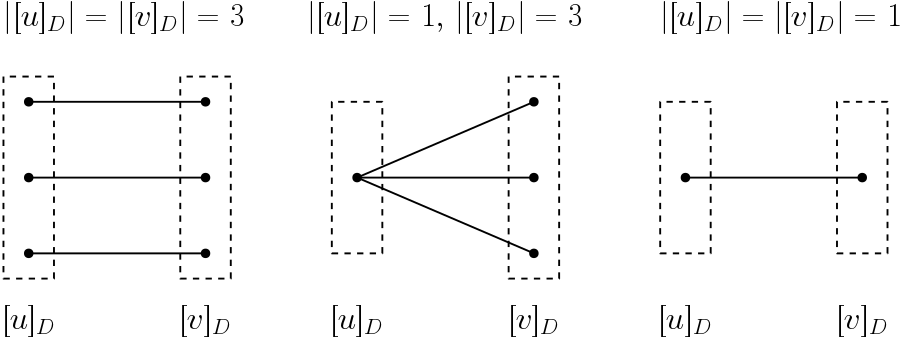
\includegraphics[scale=0.3]{assets/edgecases.png}
\caption{Three possible edge cases for Lemma~\ref{lemma:threeedges}}
\par\smallskip\noindent Original Figure~7 labels, from left to right:
\[
|[u]_D|=|[v]_D|=3;\qquad |[u]_D|=1,\ |[v]_D|=3;\qquad |[u]_D|=|[v]_D|=1.
\]
\noindent The left and right boxes in each column are labelled $[u]_D$ and $[v]_D$, respectively.
\label{fig:edgecases}
\end{figure}
Now, we again consider the equivalence classes $[v]_D$ of $V(G)$ under the relation $\sim_D$. Recall from Lemma~\ref{lemma:threeedges} that if $uv\in E(G)$ and $[u]_D\neq [v]_D$, then there are exactly three edges between the vertices in $[u]_D$ and in $[v]_D$. By Lemma~\ref{lemma:1or3}, we have $|[v]_D| = 1$ or $|[v]_D| = 3$ for each vertex $v \in V(G)$. The cases depicted in Figure~\ref{fig:edgecases} are thus the only possible edge configurations between equivalence classes. Furthermore, note that the third case in Figure~\ref{fig:edgecases} is impossible because we cannot send all three chips along a single edge at once.

Define $\sigma : V(G) \to V(G)$ to be the map which permutes the vertices of each equivalence class $[v]_D$ in the following fashion: Choose a vertex $v_1 \in V(G)$ such that $|\supp (D_{v_1})| = 3$. Such a vertex must exist because otherwise, since our graph is connected and not a single vertex, we would be in the third case of Figure~\ref{fig:edgecases}. For the unique vertices $v_1, v_2, v_3 \in [v_1]_D$, let $\sigma(v_1) = v_2$, $\sigma(v_2) = v_3$, and $\sigma(v_3) = v_1$. For each edge from a vertex in $[v_1]_D$ to a vertex in another equivalence class $[u_1]_D$, define $\sigma$ as follows. If $e = v_1u_1 \in E(G)$ with $|\supp (D_{u_1})| = 3$, then let $\sigma(u_1) = u_2$ where $u_2 \in [u_1]_D$ is the unique vertex such that $\sigma(v_1)u_2 \in E(G)$. Then we must have $\sigma(u_2) = u_3$ where $u_3$ is the unique vertex with $\sigma(v_2)u_3 \in E(G)$. On the other hand, if $|\supp (D_{u_1})| = 1$, then let $\sigma$ act as the identity on $u_1$. 

Let this process, where vertex classes induce orderings on their adjacent vertex classes, propagate outwards. If we reach a situation where a vertex class with one vertex induces an order on a vertex class with three vertices, pick some arbitrary ordering on those three vertices and define $\sigma$ accordingly. We will show that the order chosen does not matter, and that this process provides us with our desired automorphism.

\begin{prop}
\label{prop:cyclic}
The map $\sigma$ is a cyclic automorphism of order $3$ that does not fix any edge of $G$.
\end{prop}

\begin{proof}
Since our graph $G$ is connected, the propagation process induces an order on each vertex class in $G$. We now argue that we never run into the problem that the induced orderings are incompatible with each other. Suppose for the sake of contradiction that we have a vertex class $[v]_D$ with one ordering induced by an adjacent class $[u]_D$ and another ordering induced by an adjacent class $[w]_D$. It is clear that $[u]_D \neq [w]_D$ and that $| [v]_D | = 3$. However, this implies that there are at least two paths from each vertex in our original vertex class $[v_1]_D$ into $[v]_D$. Consider the divisor $D_{v}$ with $[v]_D \in \supp (D_v)$, and begin Dhar's burning algorithm at our starting vertex from $[v_1]_D$. We will show that no matter how the algorithm runs, we reach a contradiction, either to $r(D)\geq 1$ or to $[u]_D\neq [w]_D$.

Let $v_a,v_b,v_c$ be the three vertices in $[v]_D$. First, assume that at least one vertex in $[v]_D$ burns, say $v_a$. Since $G$ is $3$-vertex-connected, it is still connected after removing $v_b$ and $v_c$, so every other vertex in $G$ must burn. We also know that $\val(v_b)$ and $\val(v_c)$ are both at least $3$, and so these vertices are adjacent to at least two burning vertices. Since each has one chip, both of these vertices (and thus the entire graph) will burn. This is a contradiction, since $r(D)\geq 1$.

Now assume none of $v_a,v_b,$ and $v_c$ burns. Since there are two burning edges coming into $[v]_D$, one from $[u]_D$ and one from $[w]_D$, these burning edges must be incident to different vertices among $v_a$, $v_b$, and $v_c$; otherwise one of these vertices would burn. When the whole graph does not burn, Dhar's burning algorithm fires chips from all unburnt vertices, which moves a chip to $[u]_D$ and a chip to $[w]_D$. This yields a rank $1$ divisor of degree $3$ with support in both $[u]_D$ and $[w]_D$, a contradiction to $[u]_D\neq [w]_D$ by Lemma~\ref{lemma:distinctorbits}.

\looseness1
Having reached a contradiction in all cases, we know that the propagation process can never lead to incompatible orderings. Notice also that if $e = uv \in E(G)$, then $\sigma^{-1}(u)\sigma^{-1}(v) \in E(G)$ because $\sigma^{-1}(u) = \sigma^2(u)$ and $\sigma^{-1}(v) = \sigma^2(v)$. Hence, we have shown that $\sigma$ is an automorphism. By definition, $\sigma$ is cyclic and we have already demonstrated that $\sigma$ has order $3$. Finally, we see that $\sigma$ does not fix any edge of $G$ because we have already shown that we cannot have an edge between two equivalence classes with one vertex each (recall that the third edge case in Figure~\ref{fig:edgecases} is impossible).
\end{proof}

We may now define the same quotient morphism $\varphi: G \to G / \sim_D$ as in Section~\ref{section:multi}. However, notice that our equivalence classes of $V(G)$ can now be viewed as orbits under the action of $\sigma$. Thus, $G / \sim_D = G / \sigma$. 



\begin{prop}
\label{prop:quotient}
The quotient morphism $\varphi: G \to G / \sigma$ is harmonic and nondegenerate. Moreover, $G/\sigma$ is a tree.
\end{prop}

The proof of this proposition will be similar to an argument from the proof of Theorem~\ref{thm:multigraph}, when we showed that the quotient map from $G$ to $G/\sim_D$ was harmonic of degree $3$, and that $G/\sim_D$ was a tree.

\begin{proof} Since $\sigma$ is an automorphism, for each vertex $v \in V(G)$ such that $v \in [v]_D$, there exists some edge $e \in E(G)$ such that $v \in e$ and $\varphi(e) = [e]_D$. (Otherwise $G/\sigma$ would not be connected.) Hence, $\varphi$ is non-degenerate. To show that $\varphi$ is harmonic, fix a vertex $v \in V(G)$ and consider all edges $[e]_D \in E(G/\sigma)$ such that $\varphi(v) = [v]_D \in [e]_D$. If $\left| [v]_D \right| = 3$, then $| \{e \in E(G) : v \in e, \varphi(e) = [e]_D \}| = D_v(v) = 1$, no matter which edge $e$ we pick. On the other hand, if $\left| [v]_D \right| = 1$, then $| \{e \in E(G) : v \in e, \varphi(e) = [e]_D \}| = D_v(v) = 3$, which is also independent of our choice of $e$. Hence, $\varphi$ is harmonic. 

For any given edge $[e]_D \in E(G/\sigma)$, 
\[
|\varphi^{-1}([e]_D)| = \sum_{v \in [v]_D} |\{ e \in E(G) : v \in e, \varphi(e) = [e]_D \}| = \sum_{v \in [v]_D} D_v(v),
\]
for any choice of $[v]_D$ such that $[v]_D \in [e]_D$. Thus, $\varphi$ is a degree $3$ morphism. The same argument from the proof of Theorem~\ref{thm:multigraph} shows that $G / \sigma$ is a tree. 
\end{proof}


\begin{proof}[Proof of Theorem~\ref{thm:simpletheorem}]
We already have the equivalence of~\eqref{4.1.1} and~\eqref{4.1.2} from Theorem~\ref{thm:multigraph}. 
The implication $\eqref{4.1.1} \implies \eqref{4.1.3}$ follows from Proposition~\ref{prop:cyclic}.

For $\eqref{4.1.3} \implies \eqref{4.1.2}$, suppose that there exists a cyclic automorphism $\sigma:G\rightarrow G$ of order $3$ that does not fix any edge of $G$, such that $G/\sigma$ is a tree. We wish to show that $\varphi : G \to G/\sigma$ is a non-degenerate harmonic morphism of degree $3$. The argument for this is nearly identical to the argument from Proposition~\ref{prop:quotient}. However, the proof of harmonicity requires a few additional details. 

Fix a vertex $v \in V(G)$ and consider all edges $[e]_{D} \in E(G/\sigma)$ such that $\varphi(v) = [v]_{D} \in [e]_{D}$. Since $\sigma$ has order $3$, either $|\varphi^{-1}([v]_{D})|=3$ or $|\varphi^{-1}([v]_{D})|=1$. If $|\varphi^{-1}([v]_{D})|=3$, then we claim that $| \{e \in E(G) : v \in e, \varphi(e) = [e]_{D} \}| = 1$, no matter which edge $e$ we pick. To see this, suppose there are multiple edges $e_1=vw_1$ and $e_2=vw_2$ in this set. Then, without loss of generality, $\sigma(e_1) = e_2$ and since $v$ is not fixed under $\sigma$, we must have $\sigma(v) = w_2$. But then $\varphi$ sends $v$ and $w_2$ to the same point, so $e_2$ is mapped to a point rather than an edge, a contradiction. On the other hand, if $|\varphi^{-1}([v]_{D})|=1$, then we claim that $| \{e \in E(G) : v \in e, \varphi(e) = [e]_{D} \}| = 3$, no matter which edge $e$ we pick. This is because $\sigma$ fixes $v$ but does not fix any of its incident edges. Hence, these edges must cycle around $v$ with order $3$. We have now shown that $\varphi$ is harmonic. By the same computation as in Proposition~\ref{prop:quotient}, $\varphi$ also has degree $3$. 
\end{proof}
\begin{thebibliography}{23}
\bibitem[1]{baker} Matthew Baker, Specialization of linear systems from curves to graphs, Algebra and Number Theory 2 (2008), no. 6, 613–653.
\bibitem[2]{bn} Matthew Baker and Serguei Norine, Riemann–Roch and Abel–Jacobi theory on a finite graph, Advances in Mathematics 215 (2007), 766–788.
\bibitem[23]{db} Josse van Dobben de Bruyn, Reduced divisors and gonality in finite graphs, Bachelor’s thesis, Mathematisch Instituut, Universiteit Leiden (Netherlands), 2012.
\bibitem[14]{dhar} Deepak Dhar, Self-organized critical state of sandpile automaton models, Physical Review Letters 64 (1990), no. 14, 1613–1616.
\bibitem[4]{bs} Matthew Baker and Farbod Shokrieh, Chip-firing games, potential theory on graphs, and spanning trees, Journal of Combinatorial Theory. Series A 120 (2013), 164–182.
\bibitem[3]{bn2} Matthew Baker and Serguei Norine, Harmonic morphisms and hyperelliptic graphs, International Math Research Notices (2009), 2914–2955.
\bibitem[12]{liyau} Gunther Cornelissen, Fumiharu Kato, and Janne Kool, A combinatorial Li–Yau inequality and rational points on curves, Mathematische Annalen 361 (2015), 211–258.
\bibitem[13]{cp} Scott Corry and David Perkinson, Divisors and sandpiles: An introduction to chip-firing, Amer. Math. Soc., Providence, RI, 2018.
\end{thebibliography}
\end{document}
